\documentclass[a4paper,10pt]{scrartcl}
\usepackage[utf8]{inputenc}
\usepackage[T1]{fontenc}
\usepackage[french]{babel}
\usepackage{textcomp}
\usepackage{array,multirow}
\usepackage{amsmath,amssymb}
\usepackage{lmodern}
\usepackage{graphicx}
\usepackage[dvipsnames,svgnames]{xcolor}
\usepackage{microtype}
\usepackage{lipsum}
\usepackage{xcolor}
\usepackage{listings}
\usepackage{fancyhdr}
\usepackage{listings}
\usepackage{url}
\usepackage[T1]{fontenc}
\usepackage{natbib}
\bibliography{bib}
\pagestyle{fancy}
\renewcommand\headrulewidth{1pt}
\fancyhead[L]{Projet UML}
\fancyhead[R]{univ tln}
\renewcommand\footrulewidth{1pt}
\fancyfoot[R]{\today}
\fancyfoot[L]{Genie Logiciel}
\usepackage{hyperref}\hypersetup{colorlinks=true,linkcolor=Brown,pdfstartview=XYZ}
\begin{document}


\title{\textcolor{teal}{Genie Logiciel : Projet UML \\ Logiciel de facturation }}


\author{Ben Amira Rawia \and Lafaille Jason \and  Procureur Thomas \and Saidi Fouad  }
\date{\today}
\maketitle
\centerline{
\includegraphics[width=10cm]{ingenierie-informatique.jpg}}

\begin{center}
 

 Université de Toulon, UFR sciences et techniques
 
\textsc{\LARGE L3 Informatique }\\[1cm]
 
  
% Title
\HRule \\[0.2cm]
 {2021-2022}
\HRule\\
\end{center}

\newpage
\tableofcontents
\newpage

\section*{Introduction}
Ce compte rendu decrit la réalisation
d'un logiciel de facturation qu’un artisan  pourrait utiliser au quotidien pour gérer ses  données personnelles, clients, devis ainsi que ses factures.

\section{Presentation des membres du groupe}
{\color{olive}
Ben Amira Rawia

Lafaille Jason

Procureur Thomas

Saidi Fouad
}

\section{Specifications Logicielles}
\subsection{Partie Codage}

Ce logiciel de Facturasation est une application Web implementée avec {\color{olive}Python} et ceci grace a la micro framework open-source de développement web {\color{olive}Flask}. ce dernier est très légeret a pour objectif de garder un noyau simple mais extensible.

Flask fournit une fonction render template qui  facilitera grandement la gestion du HTML en écrivant le code {\color{olive}HTML} dans des fichiers .html .

Le langage  {\color{olive}CSS} a ete utilisé pour styliser l’application et la rendre plus attrayante en utilisant notre propre design.

\subsection{Partie UML}
pour pouvoir creer des diagrammes UML lisibles et comprehensiobles on a utilisé {\color{olive}PlantUML} qui est un outil open source permettant aux utilisateurs de créer des diagrammes à partir d'un langage de texte brut.

\subsection{Partie Maquettage}

\subsection{Travail en groupe}

Pour le travail en groupe, on a utilisé {\color{olive}GIT} pour emerger notre code. On a utilisé  la plateforme web GitHub, certain  d'entre nous ont utilisé GitBash et d'autres GithubDesktoppour faire les differents push, commit..etc .

Pour discuter de l'evolution du projet et pouvoir travailler en parallelle en dehors des seances de TP, on a utilisé {\color{olive}Discord} qui nous a permis de faire des reunions en groupe.

\section{Maquettage du logiciel}
\centerline{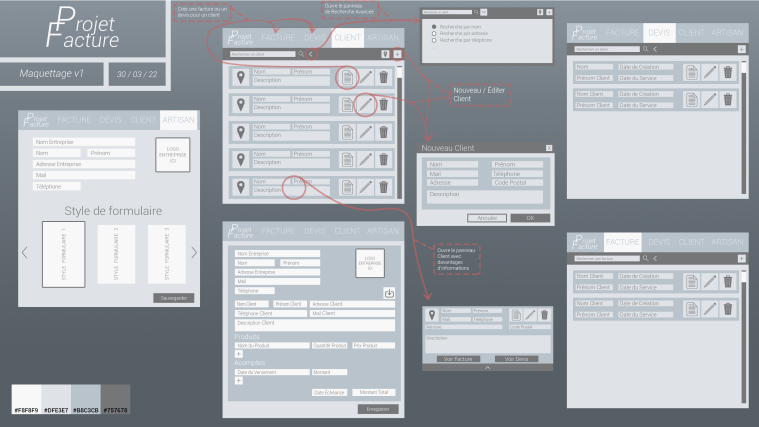
\includegraphics[width=1cm]{maquettage.png}}

\section{Diagrammes UML}
\subsection{Axe fonctionnel}
l'axe fonctionnel decrit le fonctionnement du système et capte les exigences fonctionnelles.

l'axe fonctionnel est decrit par les differents cas d'utilisation suivants : 

\centerline{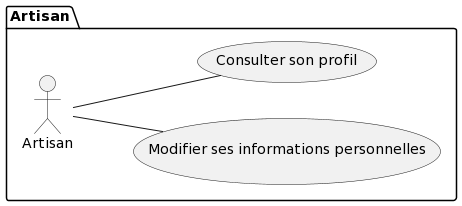
\includegraphics[width=12cm]{artisan.png}}
\centerline{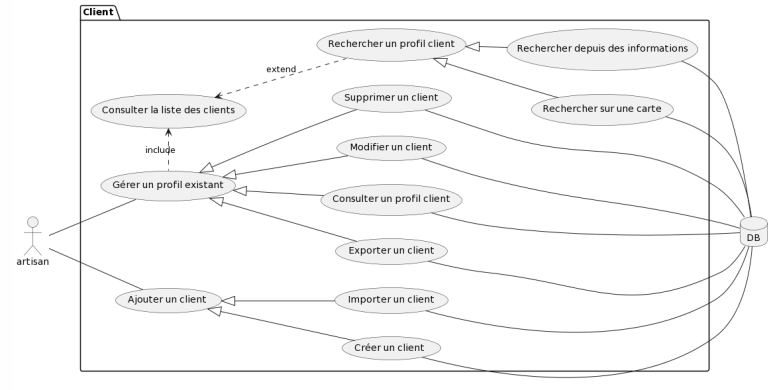
\includegraphics[width=12cm]{client.png}}
\centerline{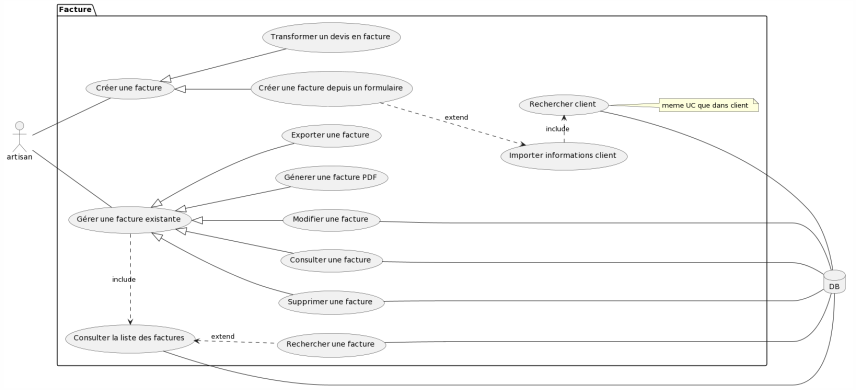
\includegraphics[width=12cm]{facture.png}}
\centerline{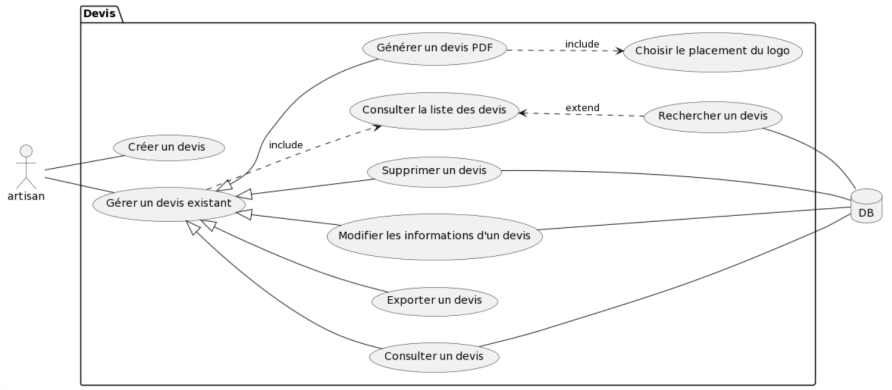
\includegraphics[width=12cm]{devis.png}}


\subsection{Axe statique}
l'axe statique Descrit les éléments du système.

\{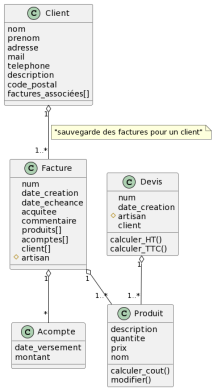
\includegraphics[width=7.5cm]{c1.png}

\{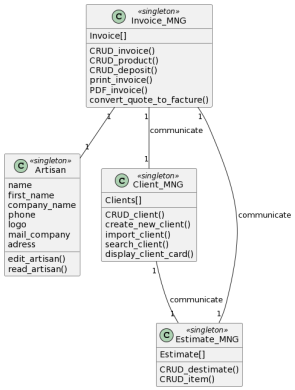
\includegraphics[width=9cm]{c2.png}

\subsection{Axe dynamique}
\centerline{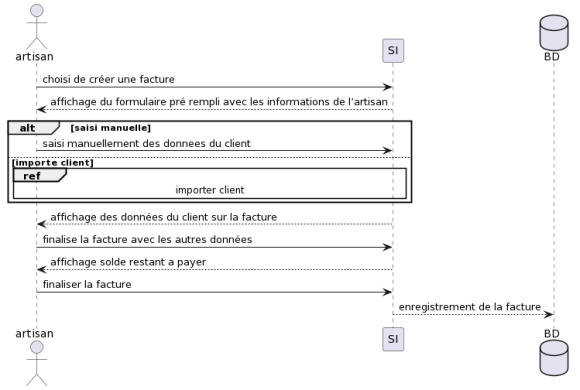
\includegraphics[width=10cm]{dyn.png}}

\section{Manuel d'instalation du logiciel}
\section{Manuel utilisateur du logiciel}
\section{Planning}


\end{document}